\section{Results}

Due to time constraints and under-budgeting, the actual sample size for this research is smaller than initially proposed. The original proposal estimated a small sample population of three to five of the most common, accessible serial printers. However, the shipment of additional printers would have taken longer than the submission deadline. All data presented is limited to available equipment at the time of reporting, the SNBC BTP-S80 serial printer.

\subsection{Device Disassembly} \label{devicedisassembly}

% \textbf{Outline}
% $\downarrow$

% \begin{itemize}
%     \item Walkthrough of documented teardown of the serial printer
%     \item Show pictures of each stage/device layers
%     \item Label pictures indicating functionality for regions of each layer (power deliver, data, I/O...)
%     \item Provide labeled key to refer in later sections
%     \item Could manufacturer increased physical security (?)
% \end{itemize}

% \textbf{The random ipsum lorem text is to gauge how much will be written when done. This will appear several times throughout the outline.}

The SNBC BTP-S80 is a common thermal printer used for providing receipts for PoS systems and immediate reporting for industrial control systems (ICS). This model features three buttons on the front face of the printer. Starting from the top: paper roll release, auto-feeding, and power button.  

\begin{figure}[ht]
    \centering
    {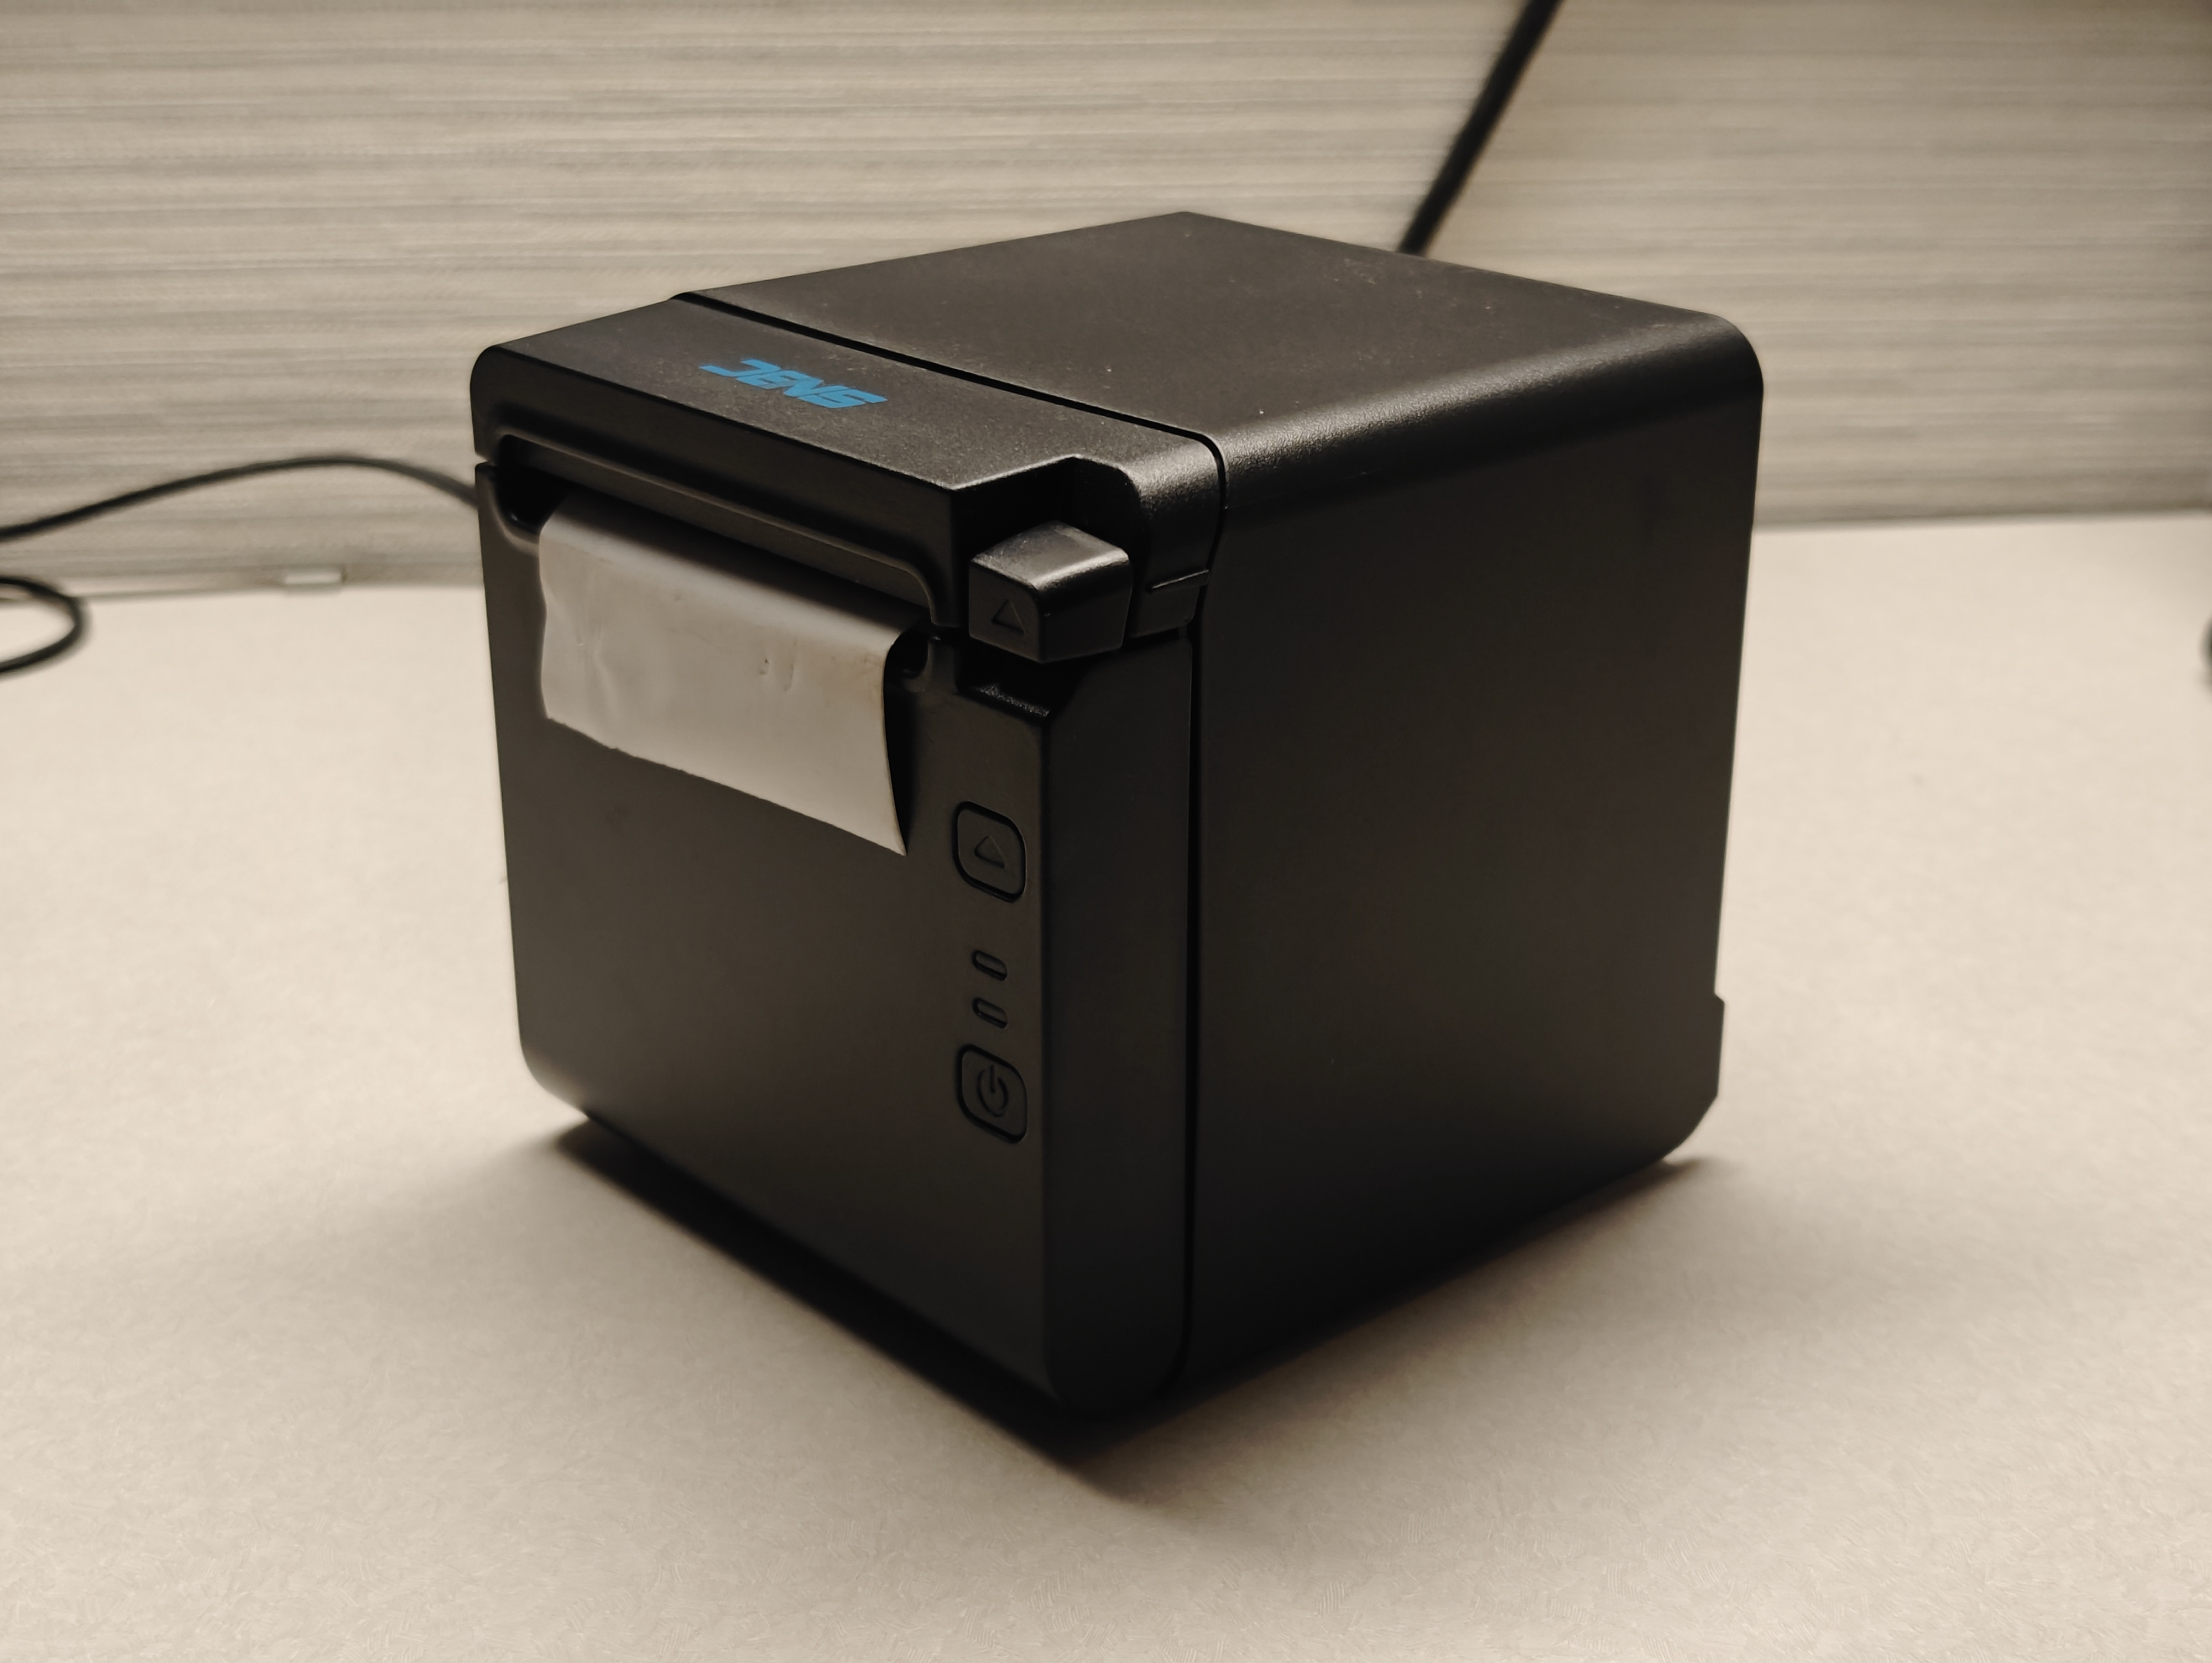
\includegraphics[width=88mm,scale=0.5]
    {Figures/Teardown/IMG20231204170511.jpg}}
    \caption{SNBC BTP-S80}
    \label{fig:snbc_btp_s80}
\end{figure}

From the rear of the device, we can see some of the available I/O. There are several ways to interface with the thermal printer. The host device can connect using an internet address via the RJ45 ethernet connector or over serial using the USB type-b and RS232. We can also see a screw on either side of the expansion card containing the RJ45 jack and RS232 connector. The manufactures website shows that this slot is interchangeable and can provide different functionality depending on the end-users needs. Some configurations are setup as shown in Figure \ref{fig:snbc_btp_s80_io}, others feature wireless adapters utilizing 2.4Ghz networking.

\begin{figure}[ht]
    \centering
    {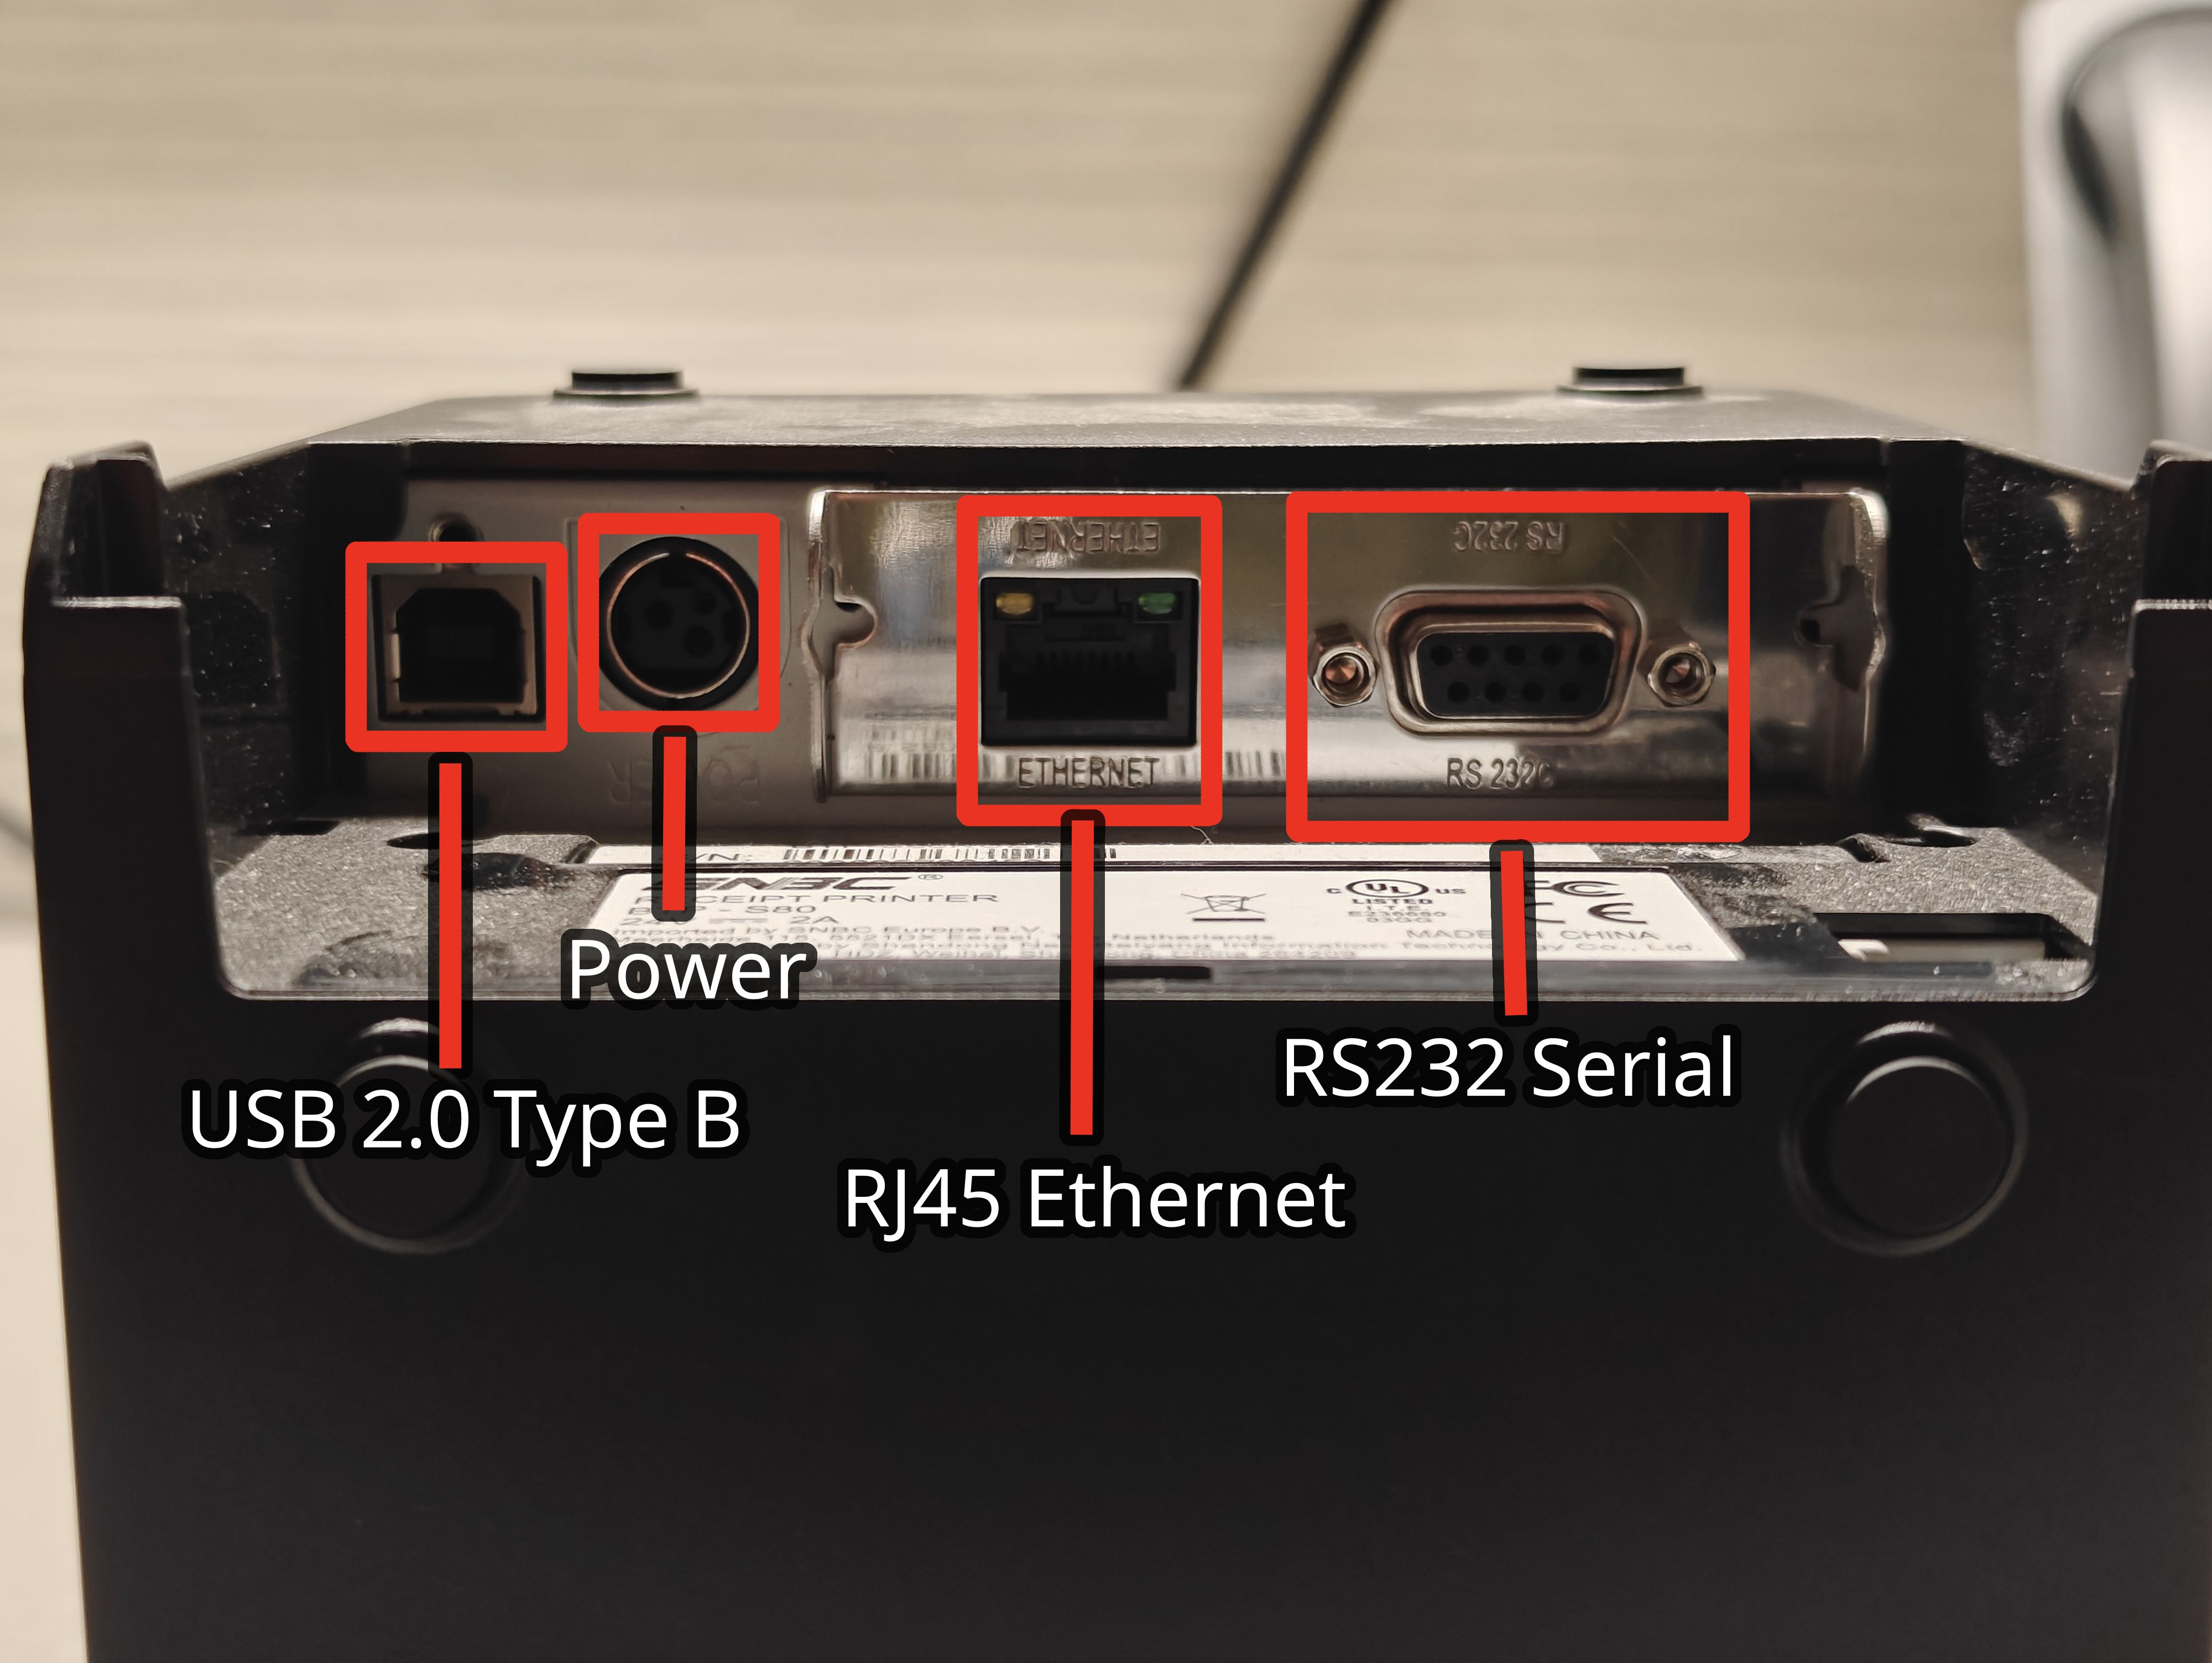
\includegraphics[width=88mm,scale=0.5]
    {Figures/Teardown/IMG20231204170442_annotated.jpg}}
    \caption{SNBC BTP-S80 labeled I/O}
    \label{fig:snbc_btp_s80_io}
\end{figure}

Removing each of the screws allows us to slide the chassis out of the outer shell. Here we can see the motherboard (leftmost) and the expansion cards (topside, right of the motherboard). The expansion cards are divided into two parts, as shown in Figure \ref{fig:snbc_btp_s80_expansion}.

\begin{figure}[ht]
    \centering
    {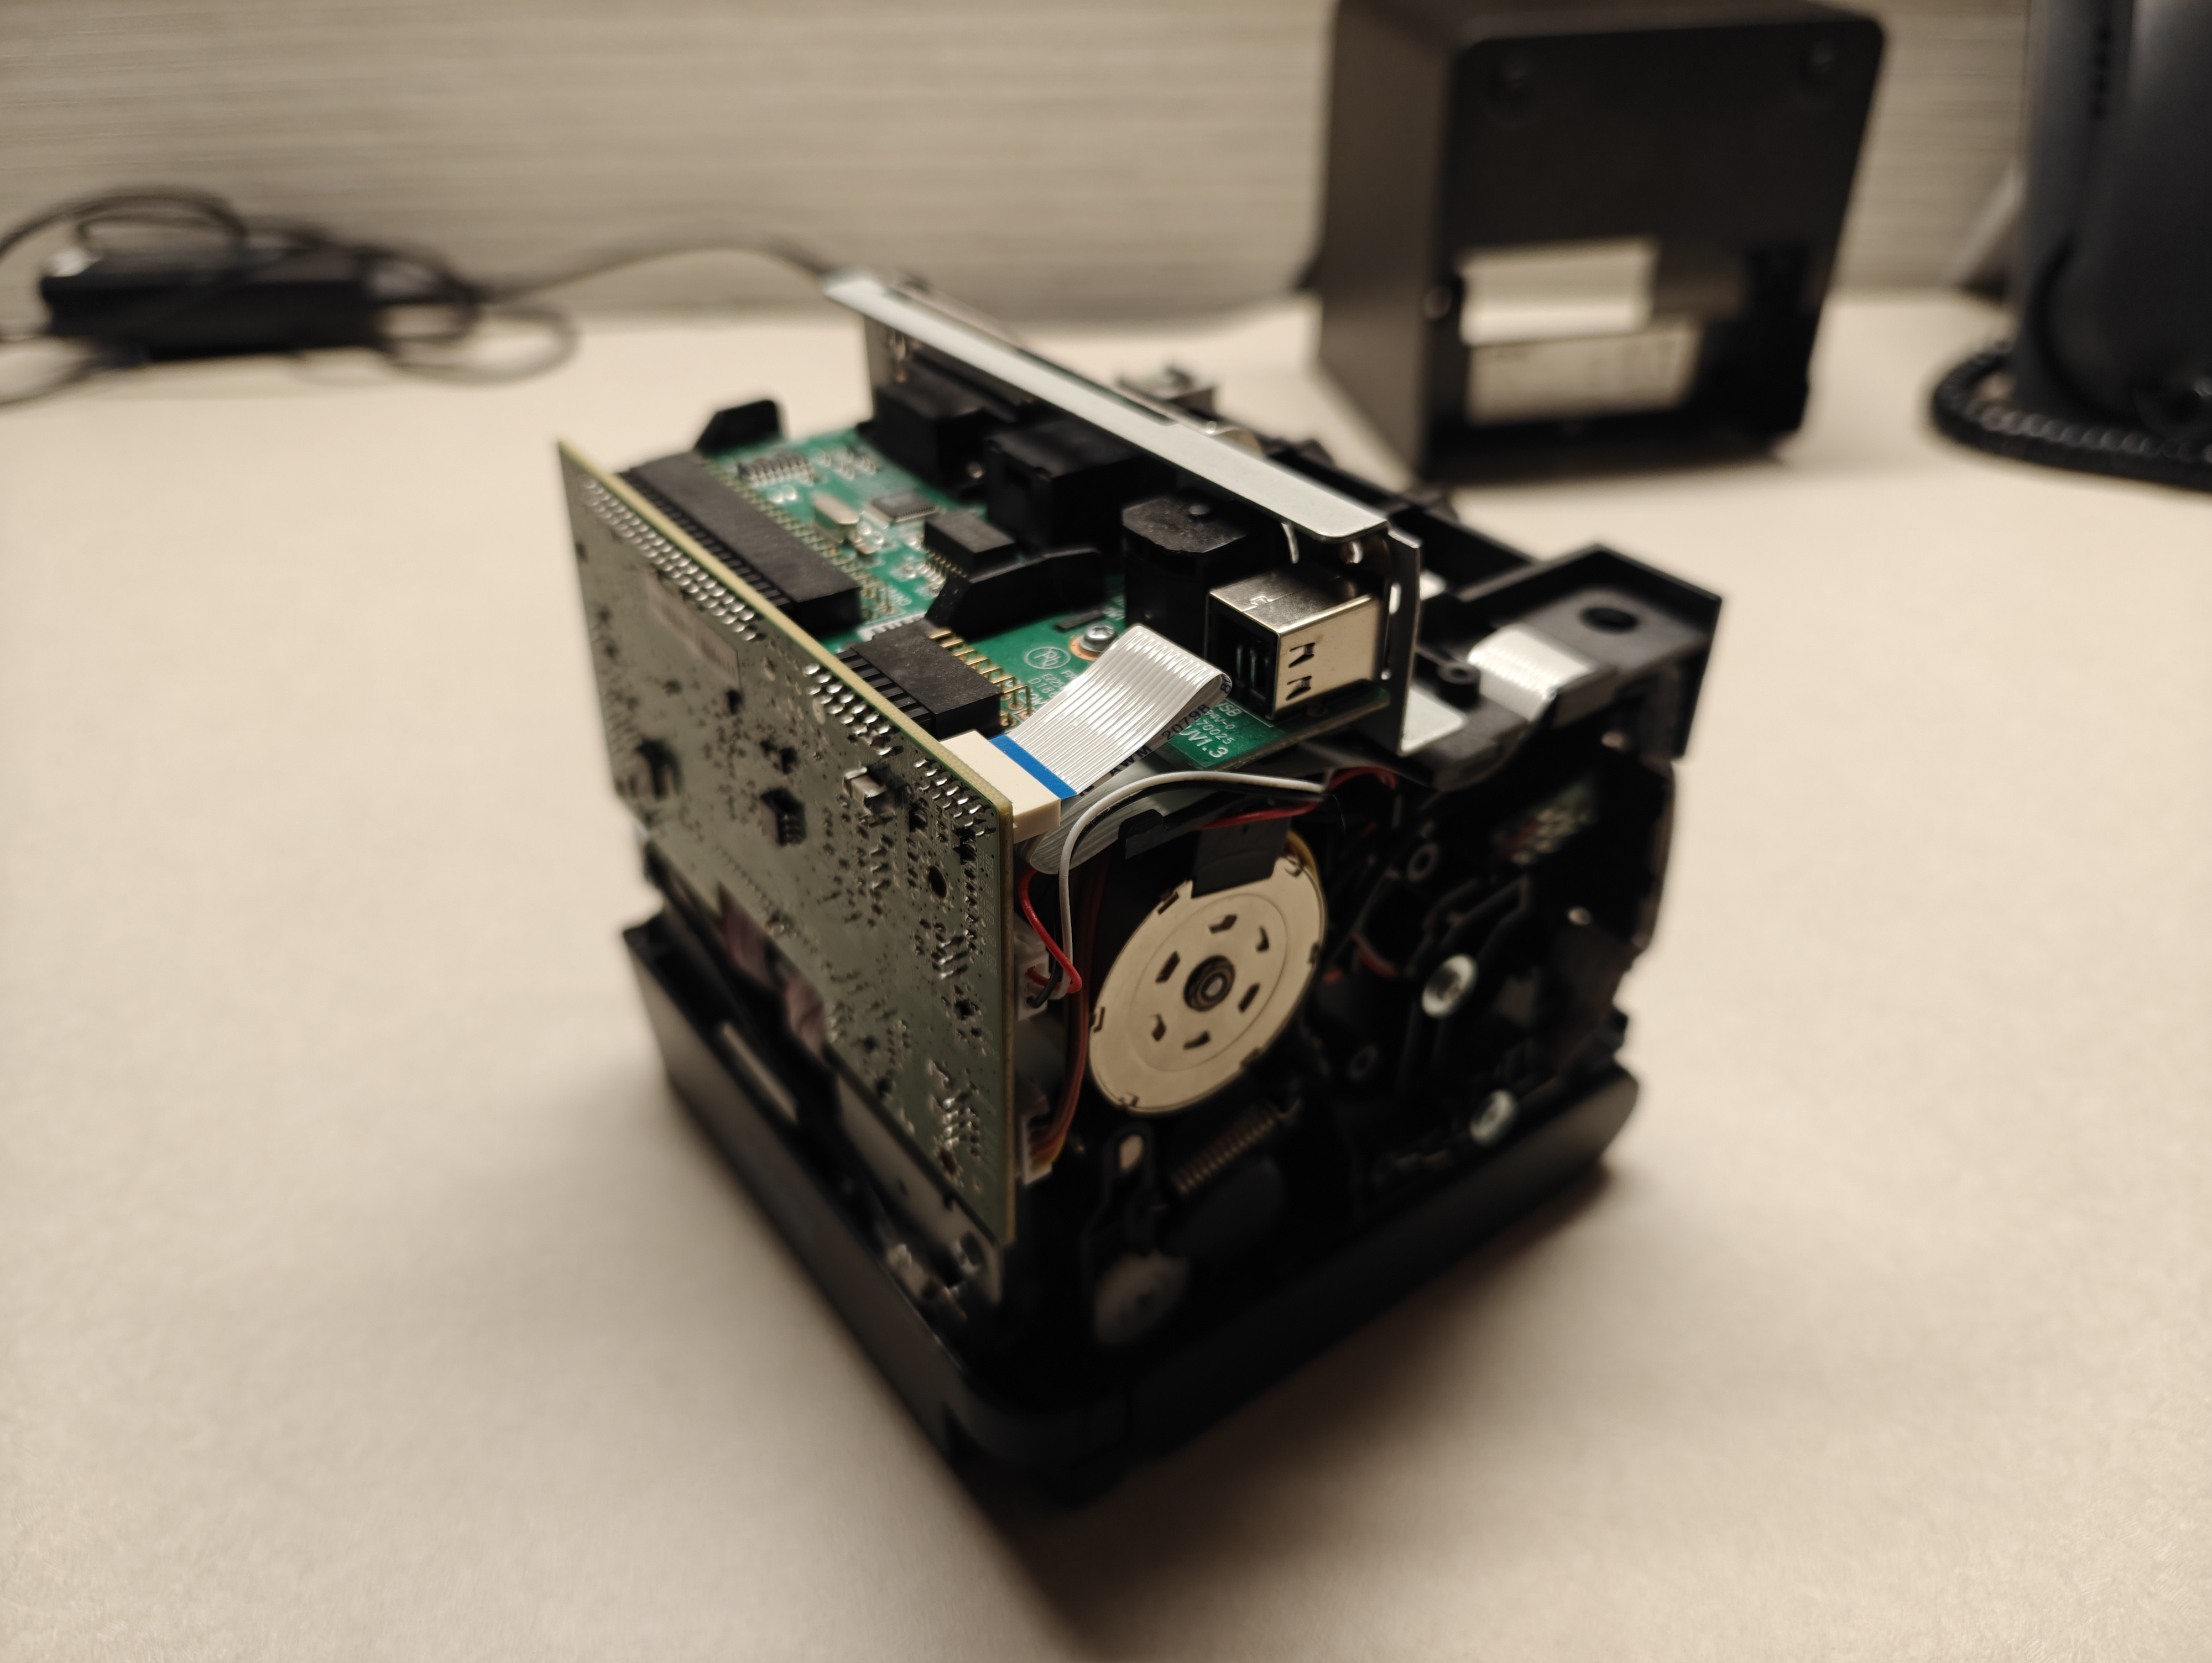
\includegraphics[width=88mm,scale=0.5]
    {Figures/Teardown/IMG20231204170938.jpg}}
    \caption{SNBC BTP-S80 inner chassis}
    \label{fig:snbc_btp_s80_chassis}
\end{figure}

The left expansion card allows the user of the device to swap networking stacks. In this configuration it features the RJ45 Ethernet and RS232 serial connector. The right expansion card provides USB connectivity and power via the barrel plug connector. 

\begin{figure}[ht]
    \centering
    {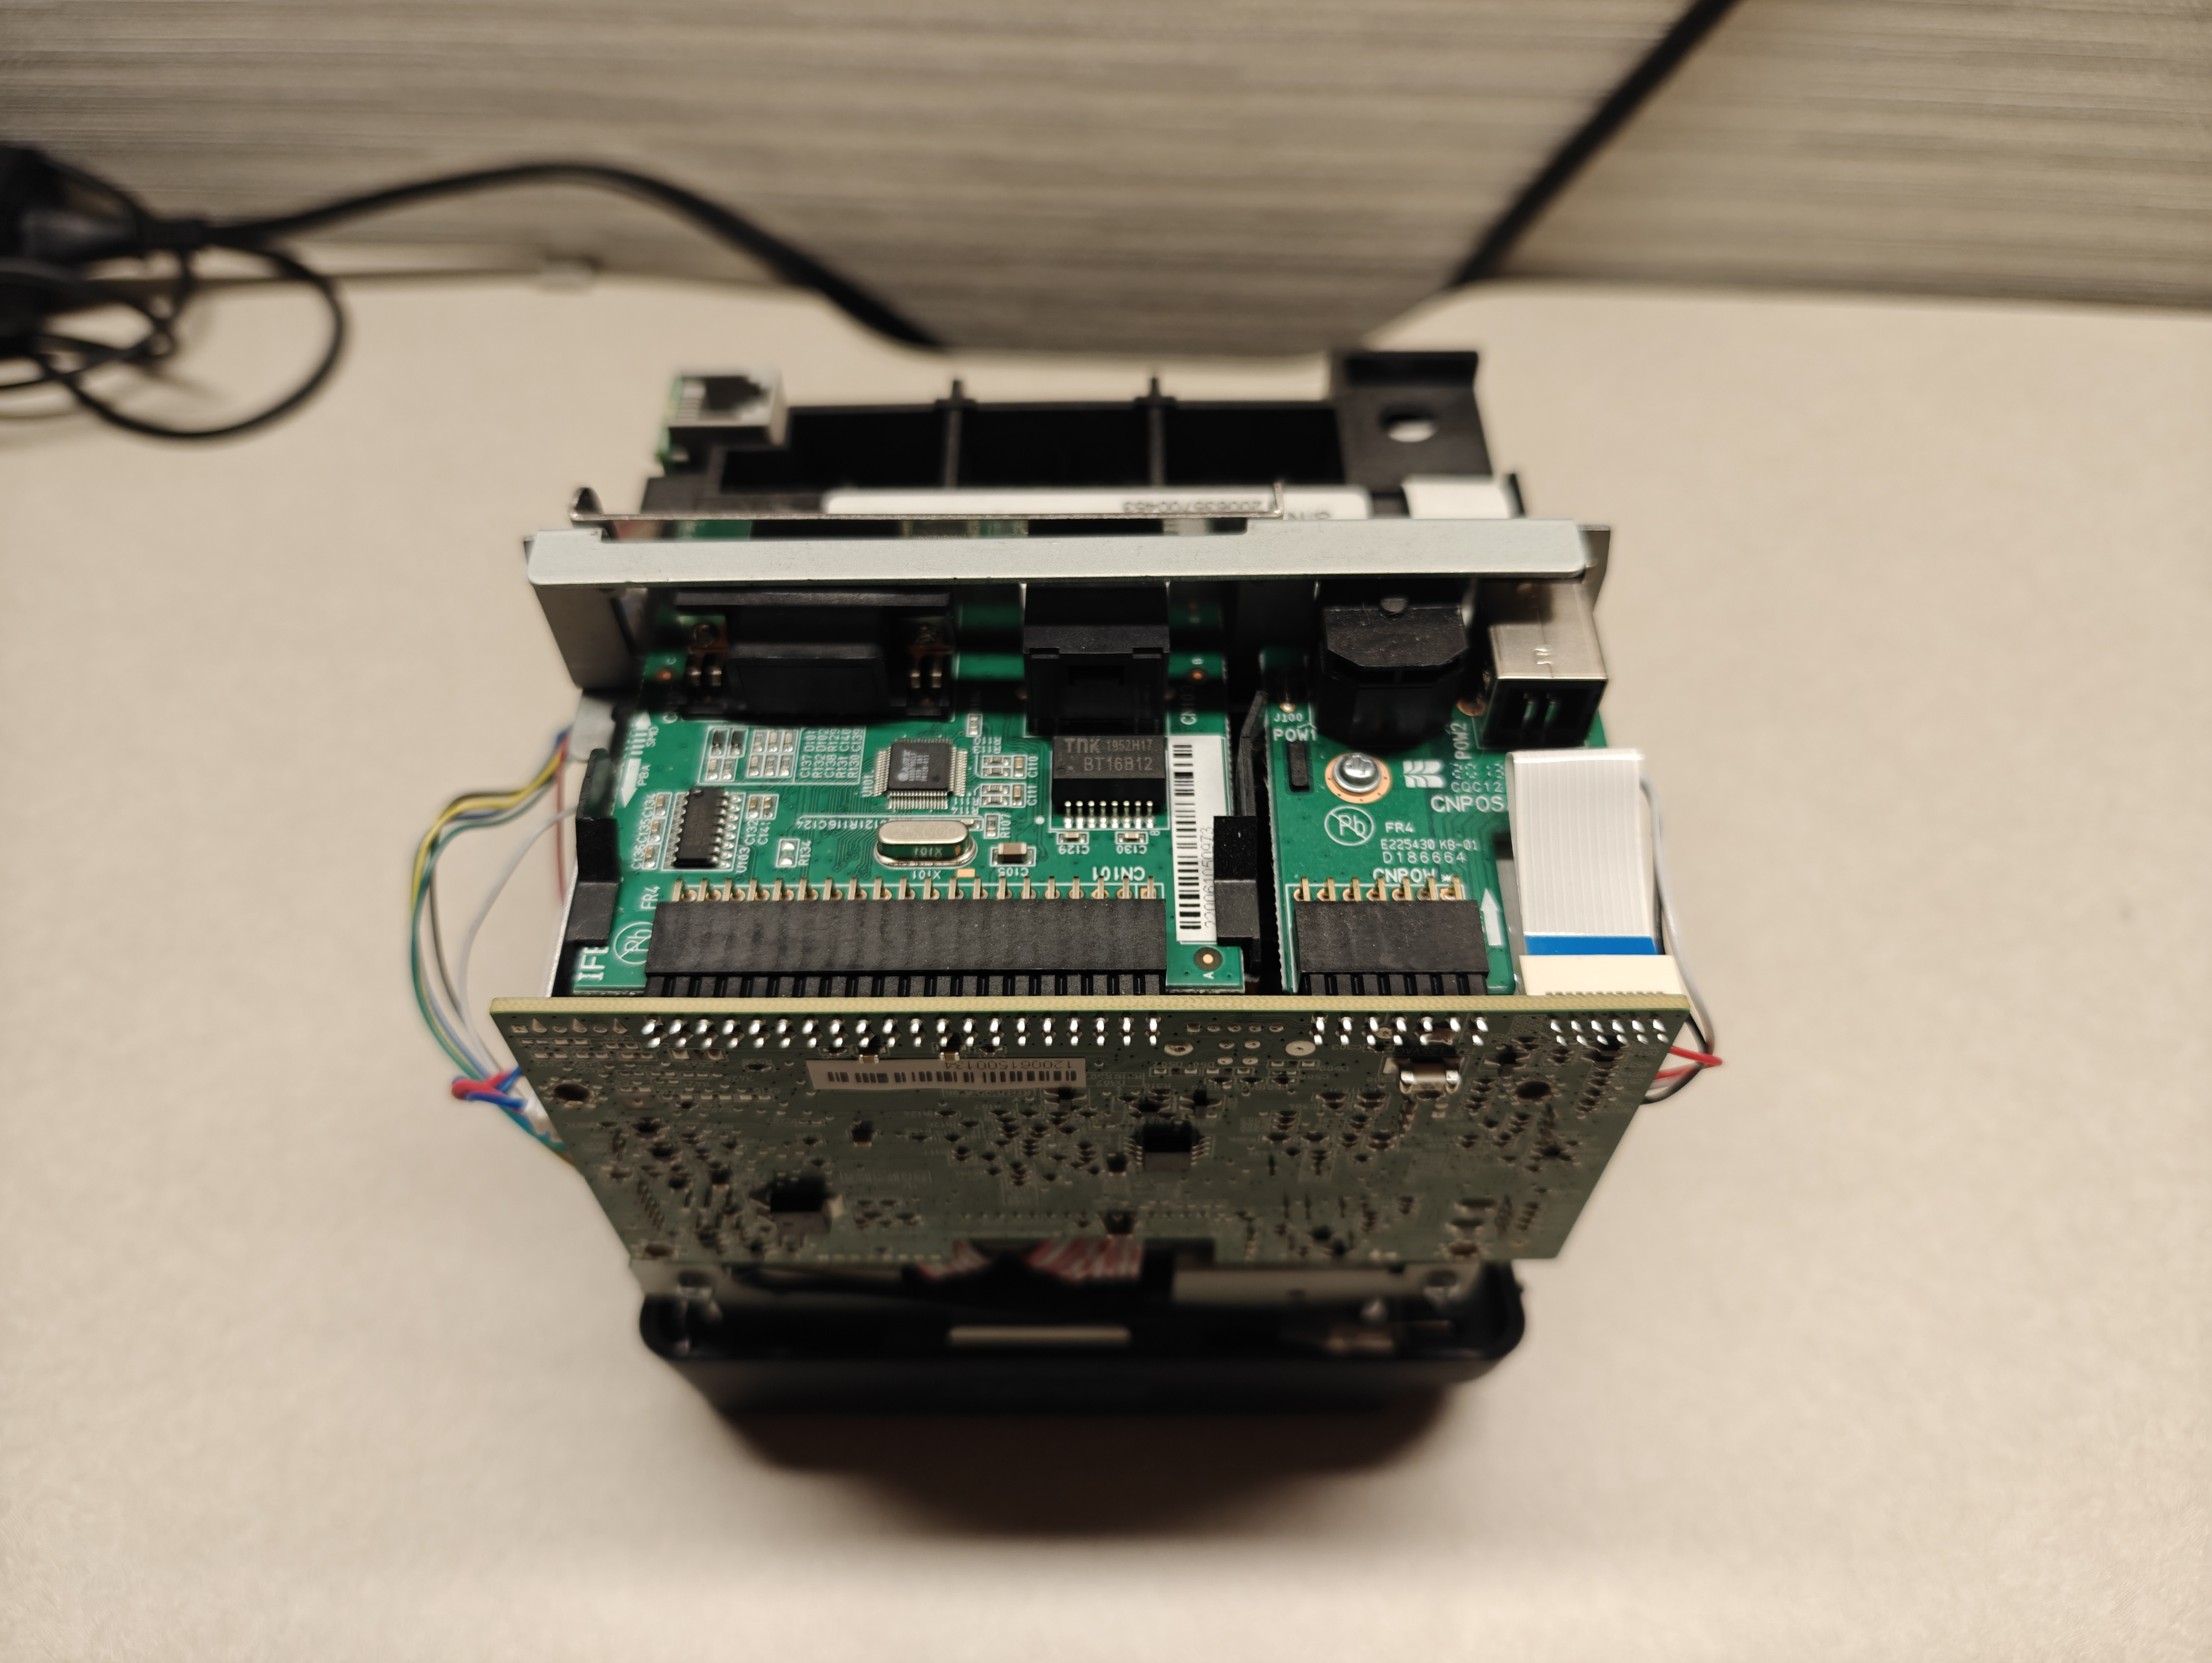
\includegraphics[width=88mm,scale=0.5]
    {Figures/Teardown/IMG20231204171002.jpg}}
    \caption{SNBC BTP-S80 expansion cards}
    \label{fig:snbc_btp_s80_expansion}
\end{figure}

The disassembly is completed after carefully disconnecting each cable, taking note of their respective connectors, and preparing the boards for component identification. There are plenty of components within the device, however, our concern is only the motherboard and two expansion cards. We are only interested in researching the components used for processing and storing data.


\subsection{Identified Components} \label{identifiedcomponents}


% \begin{itemize}
%     \item Walkthrough of documented teardown of the serial printer
% \end{itemize}

Component identification and analysis is divided into two parts. The first being analysis of the motherboard, and the second being the serial expansion card. Analysis of the power delivery and USB type-b expansion card is not necessary since it features no controllers nor any flash to analyze. In some cases, these might still be used for fuzzing and debugging because labeled connectors are provided, however, this can be ignored with most single wire debugging tools (e.g., Jtagulator or Bus Pirate).

\begin{figure}[ht]
    \centering
    {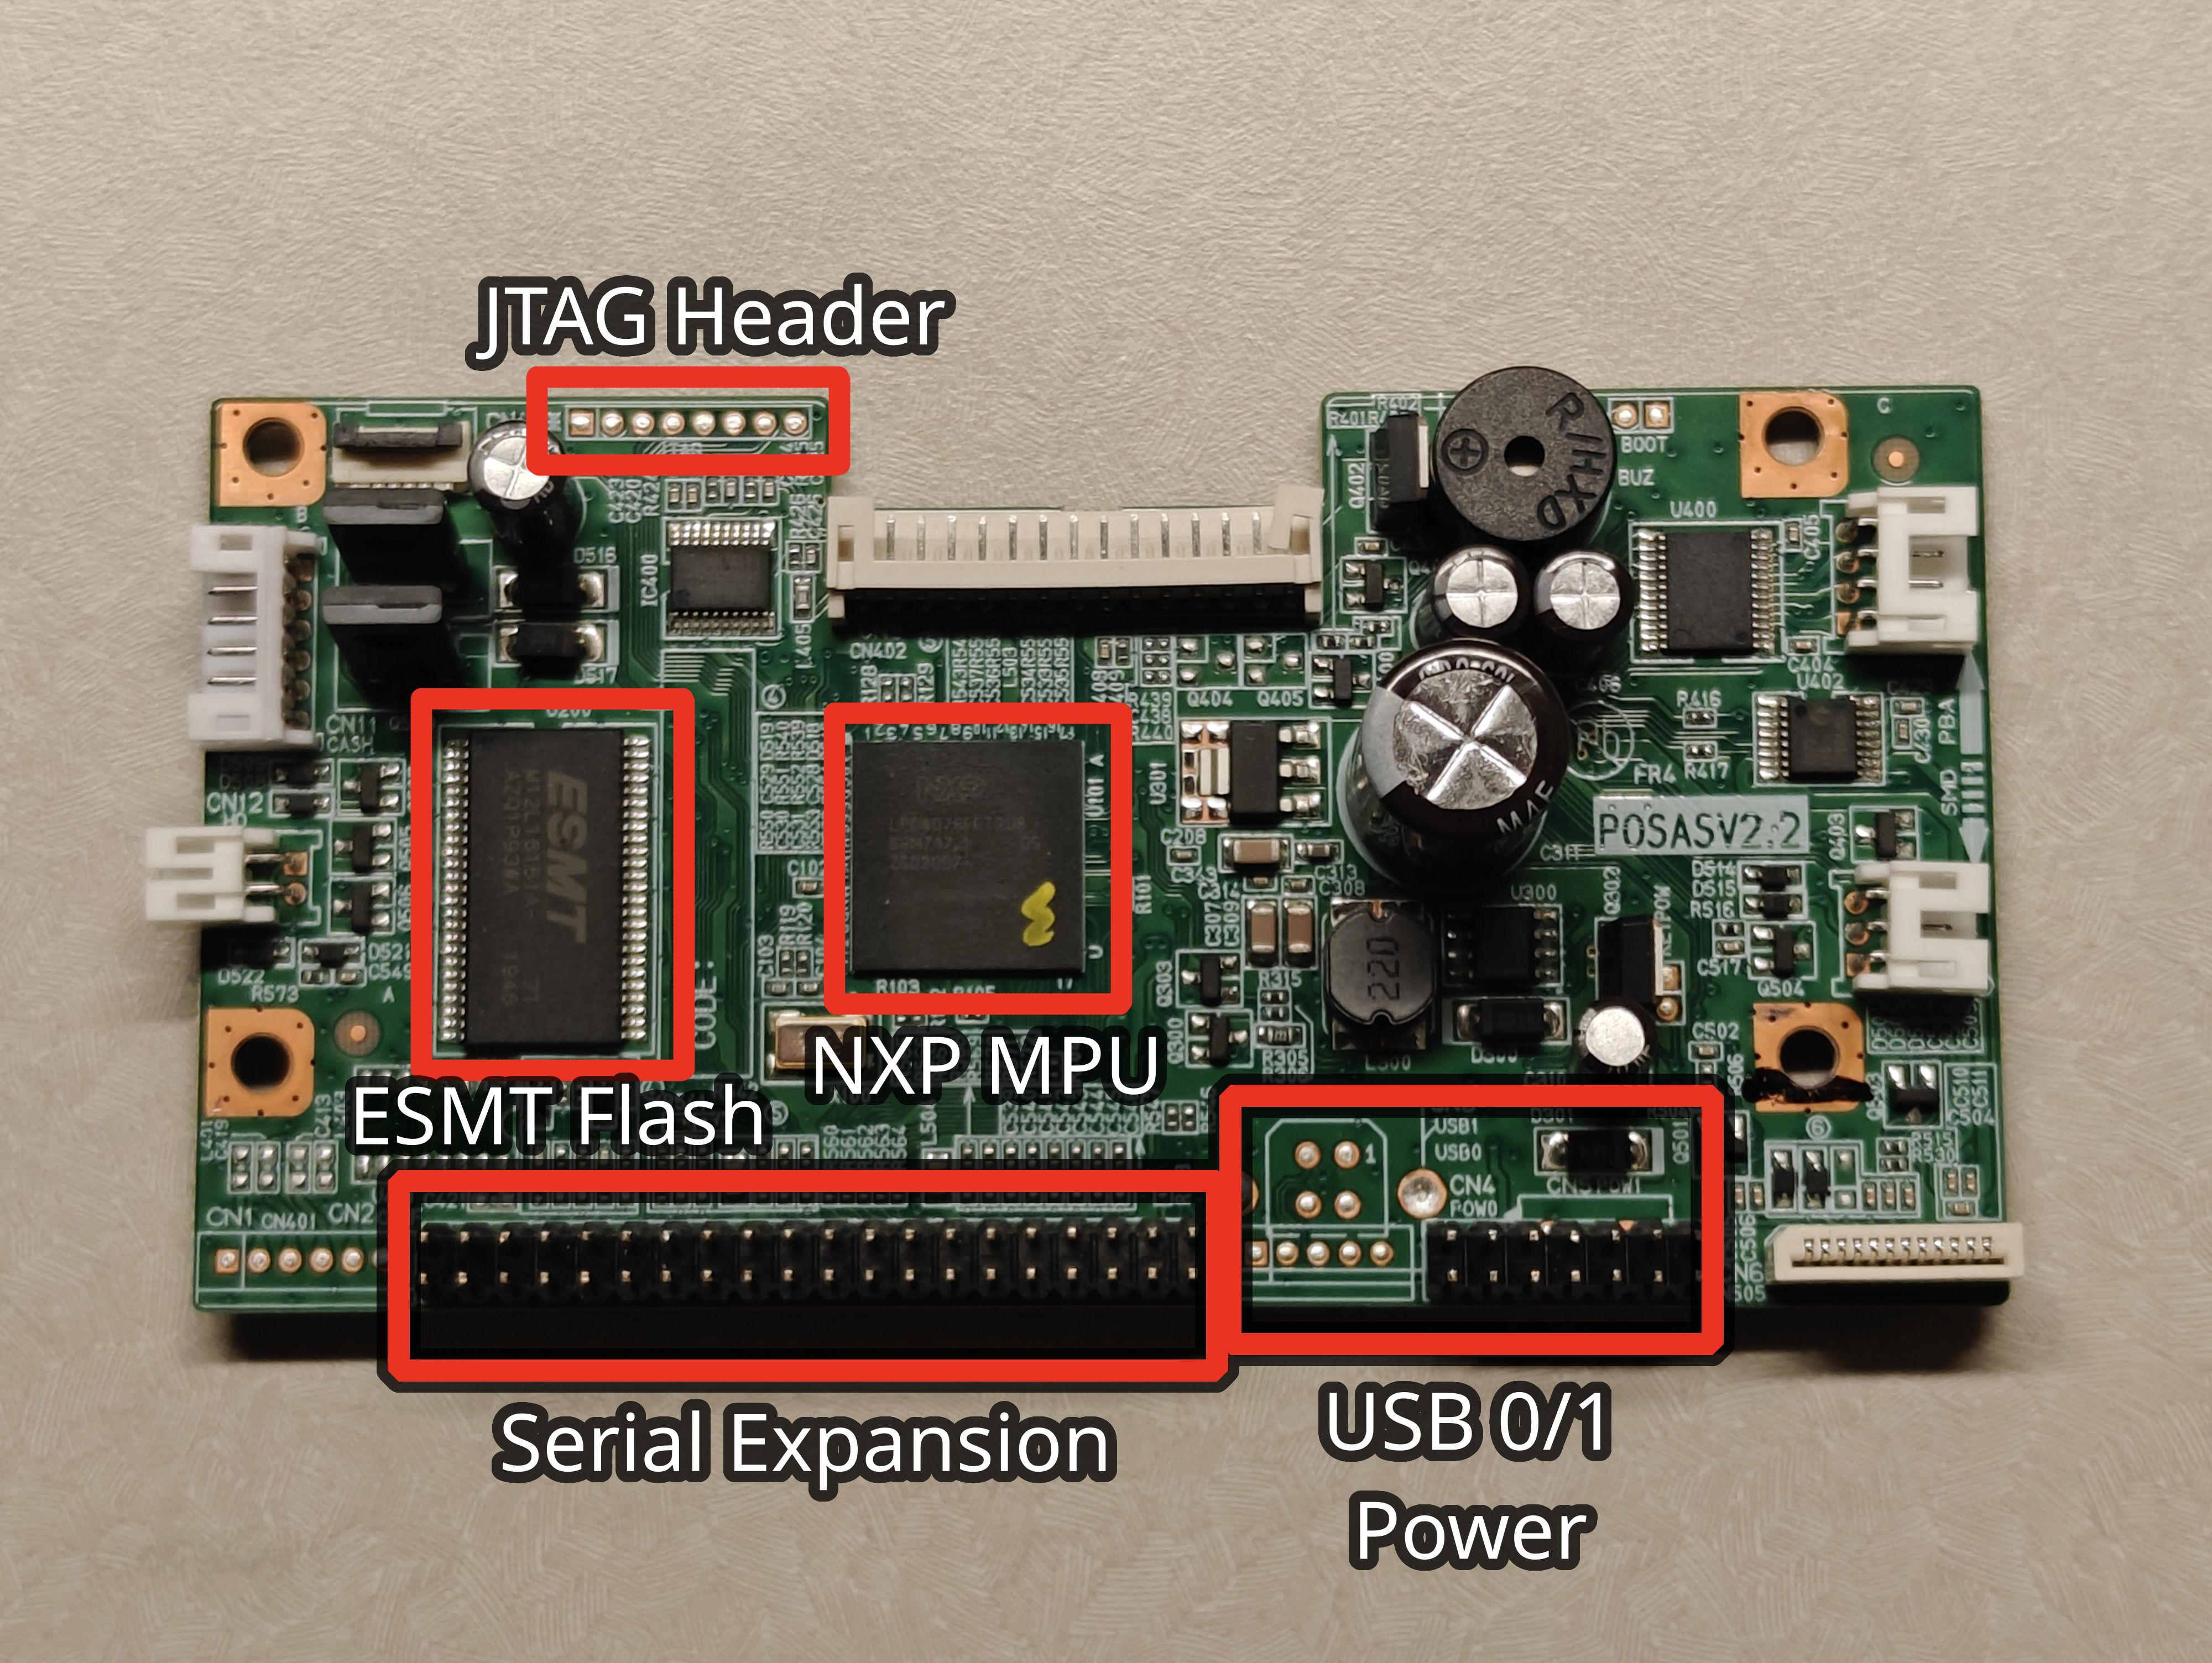
\includegraphics[width=88mm,scale=0.5]
    {Figures/Teardown/IMG20231204171516_annotated.jpg}}
    \caption{Motherboard components}
    \label{fig:snbc_btp_s80_motherboard}
\end{figure}

The list of motherboard components, as shown in Figure \ref{fig:snbc_btp_s80_motherboard}:
\begin{itemize}
    \item NXP 32-bit ARM Cortex-M4 MCU, LPC4078FET208
    \item ESMT DRAM, M12L16161A-7T
\end{itemize}

\begin{figure}[ht]
    \centering
    {\includegraphics[width=88mm,scale=0.5]
    {Figures/Teardown/IMG20231204171204_annotated.jpg}}
    \caption{Expansion card components}
    \label{fig:snbc_btp_s80_expansion_components}
\end{figure}

The list of expansion components, as shown in Figure \ref{fig:snbc_btp_s80_expansion_components}:
\begin{itemize}
    \item SIPEX RS-232 Transceiver, SP2209E
    \item ASIX Ethernet Controller, AX88796C
\end{itemize}

All of these parts can be identified by reading the labeled markings. Typically, there is a manufacturer logo, production date (e.g., YYMM), lot number, and part number. Using this information we cross reference a part database to validate the package of the component (e.g., QFP versus BGA types) and functionality. The records should tell us whether the component is the main processing unit, flash storage, or a micro-controller. Refer to Tables XX for relevant specifications regarding each component. This information aides the firmware analysis section as well as future research.

\begin{table*}
    \centering
    \label{table:LPC4078FET208}%
    \caption{NXP 32-bit ARM Cortex-M4 MCU, LPC4078FET208 \autocite{alldatasheet.comLPC4078FET208DatasheetPDF}}
    \begin{tabular}{|p{4cm}|p{12cm}|}
        \hline\rowcolor{gray!30}
    
        \textbf{Specifications} &  \\
        \hline
    
        Architecture & 32-bit ARM \\
        \hline
    
        Platform & ARM Cortex-M4 \\
        \hline
    
        Frequency & 120-MHz performance \\
        \hline
    
        Memory & 512 kB flash program memory \\
         & 96kB SRAM data memory \\
         & 4032 bytes of EEPROM data memory \\
        \hline

        Features & External Memory Controller (EMC) \\
         & General Purpose DMA Controller \\
         & Quadrature Encoder Interface \\
         & CRC calculation engine \\
         & Code Read Protection (CRP) \\
        \hline
    
        Advanced Comm. Interfaces & UART, SPIFI, I2C, USB/OTG, Ethernet, SSP \\
        \hline
    
        Debug Interfaces & JTAG, SWD \\
        \hline

        Power & Single 3.3V (2.4V to 3.6V) \\
        \hline
    
        Package format & 208-ball, TFBGA208 \\
        \hline
    
    \end{tabular}
\end{table*}

\begin{table*}
    \centering
    \label{table:M12L16161A-7T}%
    \caption{ESMT DRAM, M12L16161A-7T \autocite{alldatasheet.comM12L16161A7TDatasheetPDF}}
    \begin{tabular}{|p{4cm}|p{12cm}|}
      \hline\rowcolor{gray!30}
  
      \textbf{Specifications} &  \\
      \hline
  
      Single power supply operation & 3.3V \\
      \hline
  
      Software Features & CMOS Technology \\
      & Synchronous high data rate DRAM \\
      & LVTTL compatible with multiplexed address \\
      & Burst Read Single-bit Write operation \\
      \hline
  
      Memory architecture & Dual banks operation \\
      & 16,777,216 bits organized as 2 x 524,288 words by 16 bits\\
      \hline
  
      Package format & 50-pin, TSOP \\
      \hline
  
    \end{tabular}
\end{table*}

\begin{table*}
    \centering
    \label{table:SP2209E}%
    \caption{SIPEX High ESD Dual Port RS-232 Transceiver, SP2209E \autocite{alldatasheet.comSP2209EDatasheetPDF}}
    \begin{tabular}{|p{4cm}|p{12cm}|}
      \hline\rowcolor{gray!30}
  
      \textbf{Specifications} &  \\
      \hline
  
      Single power supply operation & 12V \\
      & Operates with +3V or +5V logic as well as standby \\
      \hline

      Comm. Interfaces & Two serial ports, Six drivers, and 10 receivers \\
      & One receiver on each port for active standby \\
      & 460kbps minimum data rate \\
      \hline

      Features & LapLink Compatible \\
      & Low EMI Emissions (EN55022) \\
      & Fast Transient Burst (EFI) Immunity (EN61000-4-2) \\
      & Pin compatible with ADM2209E \\
      \hline
  
      Package format & 38-pin, TSSOP \\
      \hline
  
    \end{tabular}
\end{table*}

\begin{table*}
    \centering
    \label{table:AX88796C}%
    \caption{ASIX Low-Power SPI or Non-PCI Ethernet Controller, AX88796C \autocite{AX88796CPdfAX88796C}}
    \begin{tabular}{|p{4cm}|p{12cm}|}
      \hline\rowcolor{gray!30}

      \textbf{Specifications} &  \\
      \hline
  
      Power & Variable voltage I/O (1.8/2.5/3.3V) \\
      & Programmable driving strength (8/16mA) \\
      \hline

      Software Features & SPI slave interface for CPU w/ SPI master \\
      & Interrupt pin with programmable timer \\
      & IPv4/IPv6 checksum offload engine \\
      & VLAN match filter \\
      & IEEE 802.3/802.3u standards for 10Base-T/100Base-TX \\
      \hline
  
      Memory & 8/16-bit SRAM-like host interface \\
      & Supports Slave-DMA to minimize CPU overhead \\
      & Burst mode read and write access over SRAM-like interface \\
      & Embeds 14KB SRAM packet buffers \\
      & Supports optional EEPROM interface for MAC storage \\
      \hline
   
      Package format & 64-pin, LQFP \\
      \hline
  
    \end{tabular}
\end{table*}


\subsection{Technical Resources} \label{technicalresources}

% List and describe datasheets and  source - AllDataSheets.com

% \textbf{Outline}
% $\downarrow$

% \begin{itemize}
%     \item List datasheets and where they were sourced
%     \item Explanation of which sites/resources and why
% \end{itemize}

All technical data and specifications sheets were procured through AllDataSheet or FindChips \autocite{ALLDATASHEETCOMElectronic,FindchipsElectronicPart}. There is a litany of other sources that can be used, however, these are the ones used by the researcher. There are no empirical reasons for using these sources instead of others, it was purely motivated by personal preference. Regardless of whichever datasheet aggregator is used, it should not harm replicability of the research.

\subsection{Firmware Analysis} \label{firmwareanalysis}

% \textbf{Outline}
% $\downarrow$

% \begin{itemize}
%     \item List bootloader information
%     \item Details about recovered memory regions (e.g., addr ranges, size, perms)
%     \item Known libraries
% \end{itemize}

As shown in Section \ref{hardwareassessment} Hardware Assessment, we can determine the correct pin layout for interfacing with the debug headers using the manufacturer datasheet. Whether or not this process is successful largely depends on the type of component packaging. In the previous example where we demonstrated reading the datasheet in relation to the pin diagram, it was possible to attach a debugger to the interface without a header prepared by the manufacturer on the device PCB. This is not possible for the SNBC BTP-S80.

Figure \ref{fig:snbc_btp_s80_motherboard} and the corresponding datasheet, shows us that the MPU uses a 208-ball thin and fine ball grid array (TFBGA) package. Unless we used a process called decapsulation or delamination it is not possible to access these pins without risking damage to the device \autocite{sanchezlopezContributionStudyElectronic2015}. The manufacturers of the BTP-S80 were kind enough to provide a JTAG debug header, as shown and labeled in Figure \ref{fig:snbc_btp_s80_motherboard}.

However, the exact pin layout is not provided. This can easily be verified manually via a multimeter and logic analyzer while referencing the manufacturer documentation. The process can be time consuming for those unfamiliar and it is recommended to use a tool such as the Jtagulator \autocite{JTAGulator2023} for enumerating the correct configuration.

With the ground and voltage reference pins validated, the researcher can connect up to 24 channels or pins. The tool will then check every permutation of the channels until an available header is identified. Using this information, we can continue with the Jtagulator or another USB debugger to continue our investigation.
